\documentclass{standalone}
\usepackage{tikz}
\usetikzlibrary{patterns, positioning}


\begin{document}
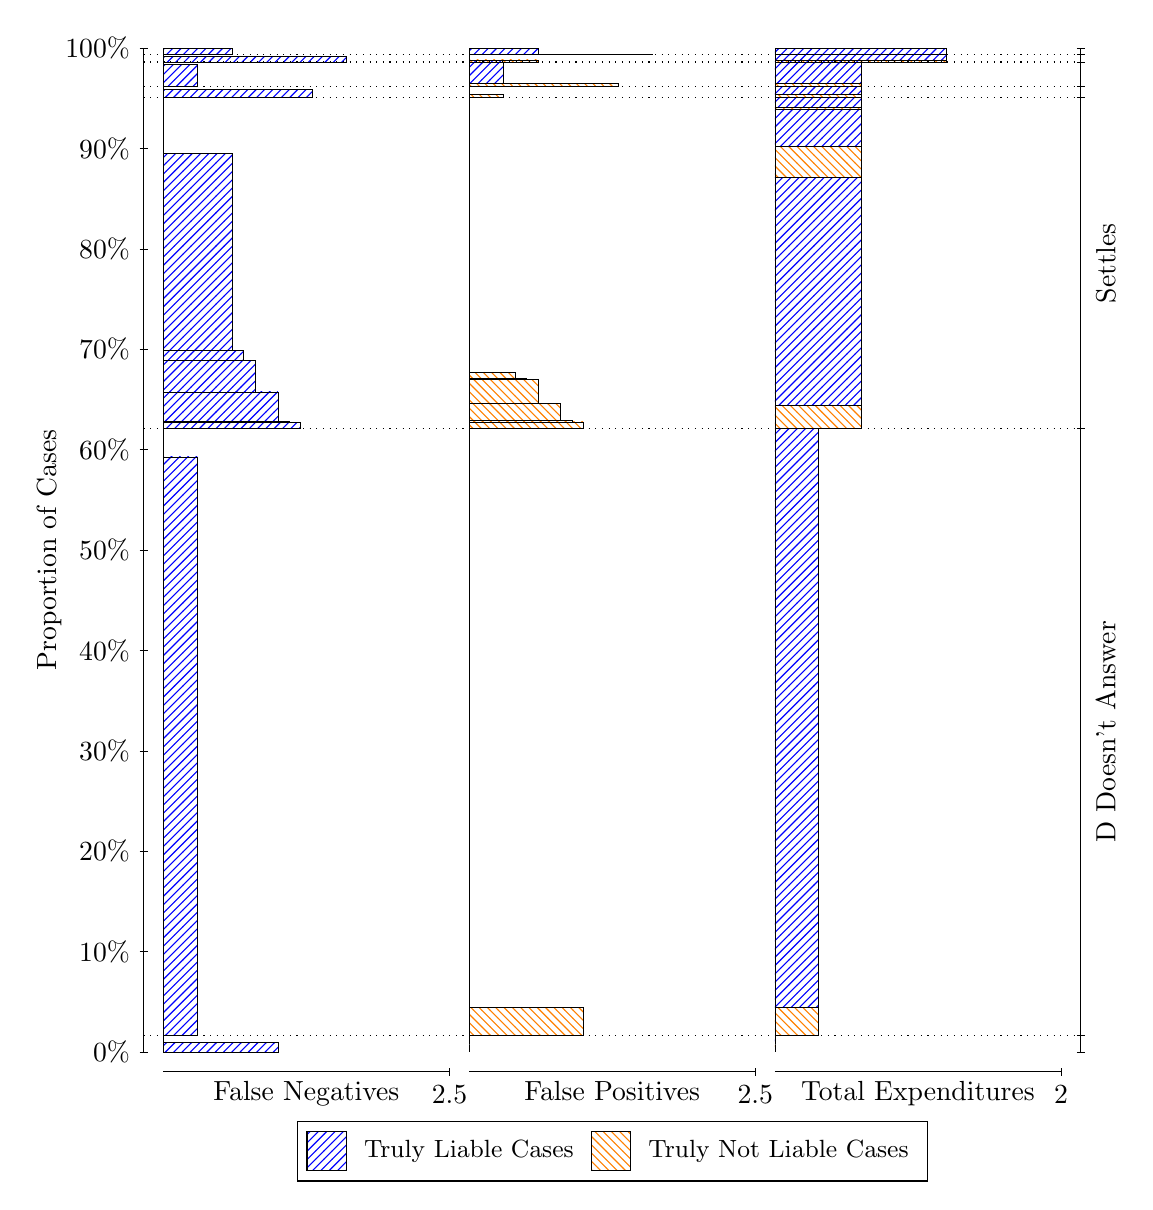
\begin{tikzpicture}
\draw[black, very thin] (1.5,1.75) -- (1.5,14.5);
\node[rotate=90, text=black, anchor=center] at (0.3, 8.125) {Proportion of Cases};
\draw[black, very thin] (1.45,1.75) -- (1.55,1.75);
\node[text=black, anchor=east] at (1.45, 1.75) {0\%};
\draw[black, very thin] (1.45,3.025) -- (1.55,3.025);
\node[text=black, anchor=east] at (1.45, 3.025) {10\%};
\draw[black, very thin] (1.45,4.3) -- (1.55,4.3);
\node[text=black, anchor=east] at (1.45, 4.3) {20\%};
\draw[black, very thin] (1.45,5.575) -- (1.55,5.575);
\node[text=black, anchor=east] at (1.45, 5.575) {30\%};
\draw[black, very thin] (1.45,6.85) -- (1.55,6.85);
\node[text=black, anchor=east] at (1.45, 6.85) {40\%};
\draw[black, very thin] (1.45,8.125) -- (1.55,8.125);
\node[text=black, anchor=east] at (1.45, 8.125) {50\%};
\draw[black, very thin] (1.45,9.4) -- (1.55,9.4);
\node[text=black, anchor=east] at (1.45, 9.4) {60\%};
\draw[black, very thin] (1.45,10.675) -- (1.55,10.675);
\node[text=black, anchor=east] at (1.45, 10.675) {70\%};
\draw[black, very thin] (1.45,11.95) -- (1.55,11.95);
\node[text=black, anchor=east] at (1.45, 11.95) {80\%};
\draw[black, very thin] (1.45,13.225) -- (1.55,13.225);
\node[text=black, anchor=east] at (1.45, 13.225) {90\%};
\draw[black, very thin] (1.45,14.5) -- (1.55,14.5);
\node[text=black, anchor=east] at (1.45, 14.5) {100\%};

\draw[black, very thin] (13.4,1.75) -- (13.4,14.5);
\draw[black, very thin] (13.35,1.75) -- (13.45,1.75);
\node[anchor=west] at (13.35, 1.75) {};
\draw[black, very thin] (13.35,1.9599) -- (13.45,1.9599);
\node[anchor=west] at (13.35, 1.9599) {};
\draw[black, very thin] (13.35,9.6665) -- (13.45,9.6665);
\node[anchor=west] at (13.35, 9.6665) {};
\draw[black, very thin] (13.35,13.87) -- (13.45,13.87);
\node[anchor=west] at (13.35, 13.87) {};
\draw[black, very thin] (13.35,14.015) -- (13.45,14.015);
\node[anchor=west] at (13.35, 14.015) {};
\draw[black, very thin] (13.35,14.323) -- (13.45,14.323);
\node[anchor=west] at (13.35, 14.323) {};
\draw[black, very thin] (13.35,14.417) -- (13.45,14.417);
\node[anchor=west] at (13.35, 14.417) {};
\draw[black, very thin] (13.35,14.5) -- (13.45,14.5);
\node[anchor=west] at (13.35, 14.5) {};

\draw[black, very thin, pattern color=blue, pattern=north east lines] (1.75,1.75) rectangle (3.2033,1.867);
\draw[black, very thin, pattern color=orange, pattern=north west lines] (1.75,1.867) rectangle (1.75,1.9599);
\draw[black, very thin, pattern color=blue, pattern=north east lines] (1.75,1.9599) rectangle (2.186,9.3084);
\draw[black, very thin, pattern color=orange, pattern=north west lines] (1.75,9.3084) rectangle (1.75,9.6665);
\draw[black, very thin, pattern color=blue, pattern=north east lines] (1.75,9.6665) rectangle (3.494,9.7486);
\draw[black, very thin, pattern color=blue, pattern=north east lines] (1.75,9.7486) rectangle (3.3487,9.7557);
\draw[black, very thin, pattern color=blue, pattern=north east lines] (1.75,9.7557) rectangle (3.2033,10.134);
\draw[black, very thin, pattern color=blue, pattern=north east lines] (1.75,10.134) rectangle (2.9127,10.532);
\draw[black, very thin, pattern color=blue, pattern=north east lines] (1.75,10.532) rectangle (2.7673,10.66);
\draw[black, very thin, pattern color=blue, pattern=north east lines] (1.75,10.66) rectangle (2.622,13.158);
\draw[black, very thin, pattern color=orange, pattern=north west lines] (1.75,13.158) rectangle (1.75,13.87);
\draw[black, very thin, pattern color=blue, pattern=north east lines] (1.75,13.87) rectangle (3.6393,13.971);
\draw[black, very thin, pattern color=orange, pattern=north west lines] (1.75,13.971) rectangle (1.75,14.015);
\draw[black, very thin, pattern color=blue, pattern=north east lines] (1.75,14.015) rectangle (2.186,14.288);
\draw[black, very thin, pattern color=orange, pattern=north west lines] (1.75,14.288) rectangle (1.75,14.323);
\draw[black, very thin, pattern color=blue, pattern=north east lines] (1.75,14.323) rectangle (4.0753,14.39);
\draw[black, very thin, pattern color=orange, pattern=north west lines] (1.75,14.39) rectangle (1.75,14.417);
\draw[black, very thin, pattern color=blue, pattern=north east lines] (1.75,14.417) rectangle (2.622,14.493);
\draw[black, very thin, pattern color=orange, pattern=north west lines] (1.75,14.493) rectangle (1.75,14.5);
\draw[black, very thin, pattern color=orange, pattern=north west lines] (5.6333,1.75) rectangle (5.6333,1.843);
\draw[black, very thin, pattern color=blue, pattern=north east lines] (5.6333,1.843) rectangle (5.6333,1.9599);
\draw[black, very thin, pattern color=orange, pattern=north west lines] (5.6333,1.9599) rectangle (7.0867,2.318);
\draw[black, very thin, pattern color=blue, pattern=north east lines] (5.6333,2.318) rectangle (5.6333,9.6665);
\draw[black, very thin, pattern color=orange, pattern=north west lines] (5.6333,9.6665) rectangle (7.0867,9.752);
\draw[black, very thin, pattern color=orange, pattern=north west lines] (5.6333,9.752) rectangle (6.9413,9.7746);
\draw[black, very thin, pattern color=orange, pattern=north west lines] (5.6333,9.7746) rectangle (6.796,9.9835);
\draw[black, very thin, pattern color=orange, pattern=north west lines] (5.6333,9.9835) rectangle (6.5053,10.296);
\draw[black, very thin, pattern color=orange, pattern=north west lines] (5.6333,10.296) rectangle (6.36,10.301);
\draw[black, very thin, pattern color=orange, pattern=north west lines] (5.6333,10.301) rectangle (6.2147,10.378);
\draw[black, very thin, pattern color=blue, pattern=north east lines] (5.6333,10.378) rectangle (5.6333,13.87);
\draw[black, very thin, pattern color=orange, pattern=north west lines] (5.6333,13.87) rectangle (6.0693,13.914);
\draw[black, very thin, pattern color=blue, pattern=north east lines] (5.6333,13.914) rectangle (5.6333,14.015);
\draw[black, very thin, pattern color=orange, pattern=north west lines] (5.6333,14.015) rectangle (7.5227,14.05);
\draw[black, very thin, pattern color=blue, pattern=north east lines] (5.6333,14.05) rectangle (6.0693,14.323);
\draw[black, very thin, pattern color=orange, pattern=north west lines] (5.6333,14.323) rectangle (6.5053,14.35);
\draw[black, very thin, pattern color=blue, pattern=north east lines] (5.6333,14.35) rectangle (5.6333,14.417);
\draw[black, very thin, pattern color=orange, pattern=north west lines] (5.6333,14.417) rectangle (7.9587,14.424);
\draw[black, very thin, pattern color=blue, pattern=north east lines] (5.6333,14.424) rectangle (6.5053,14.5);
\draw[black, very thin, pattern color=orange, pattern=north west lines] (9.5167,1.75) rectangle (9.5167,1.843);
\draw[black, very thin, pattern color=blue, pattern=north east lines] (9.5167,1.843) rectangle (9.5167,1.9599);
\draw[black, very thin, pattern color=orange, pattern=north west lines] (9.5167,1.9599) rectangle (10.062,2.318);
\draw[black, very thin, pattern color=blue, pattern=north east lines] (9.5167,2.318) rectangle (10.062,9.6665);
\draw[black, very thin, pattern color=orange, pattern=north west lines] (9.5167,9.6665) rectangle (10.607,9.9609);
\draw[black, very thin, pattern color=blue, pattern=north east lines] (9.5167,9.9609) rectangle (10.607,12.858);
\draw[black, very thin, pattern color=orange, pattern=north west lines] (9.5167,12.858) rectangle (10.607,13.253);
\draw[black, very thin, pattern color=blue, pattern=north east lines] (9.5167,13.253) rectangle (10.607,13.72);
\draw[black, very thin, pattern color=orange, pattern=north west lines] (9.5167,13.72) rectangle (10.607,13.742);
\draw[black, very thin, pattern color=blue, pattern=north east lines] (9.5167,13.742) rectangle (10.607,13.87);
\draw[black, very thin, pattern color=orange, pattern=north west lines] (9.5167,13.87) rectangle (10.607,13.914);
\draw[black, very thin, pattern color=blue, pattern=north east lines] (9.5167,13.914) rectangle (10.607,14.015);
\draw[black, very thin, pattern color=orange, pattern=north west lines] (9.5167,14.015) rectangle (10.607,14.05);
\draw[black, very thin, pattern color=blue, pattern=north east lines] (9.5167,14.05) rectangle (10.607,14.323);
\draw[black, very thin, pattern color=orange, pattern=north west lines] (9.5167,14.323) rectangle (11.697,14.35);
\draw[black, very thin, pattern color=blue, pattern=north east lines] (9.5167,14.35) rectangle (11.697,14.417);
\draw[black, very thin, pattern color=orange, pattern=north west lines] (9.5167,14.417) rectangle (11.697,14.424);
\draw[black, very thin, pattern color=blue, pattern=north east lines] (9.5167,14.424) rectangle (11.697,14.5);
\draw[black, dotted] (1.5,1.9599) -- (13.4,1.9599);
\draw[black, dotted] (1.5,9.6665) -- (13.4,9.6665);
\draw[black, dotted] (1.5,13.87) -- (13.4,13.87);
\draw[black, dotted] (1.5,14.015) -- (13.4,14.015);
\draw[black, dotted] (1.5,14.323) -- (13.4,14.323);
\draw[black, dotted] (1.5,14.417) -- (13.4,14.417);
\draw[black, very thin] (1.75,1.5) -- (5.3833,1.5);
\node[text=black, anchor=north] at (3.5667, 1.5) {False Negatives};
\draw[black, very thin] (5.3833,1.45) -- (5.3833,1.55);
\node[text=black, anchor=north] at (5.3833, 1.45) {2.5};

\draw[black, very thin] (5.6333,1.5) -- (9.2667,1.5);
\node[text=black, anchor=north] at (7.45, 1.5) {False Positives};
\draw[black, very thin] (9.2667,1.45) -- (9.2667,1.55);
\node[text=black, anchor=north] at (9.2667, 1.45) {2.5};

\draw[black, very thin] (9.5167,1.5) -- (13.15,1.5);
\node[text=black, anchor=north] at (11.333, 1.5) {Total Expenditures};
\draw[black, very thin] (13.15,1.45) -- (13.15,1.55);
\node[text=black, anchor=north] at (13.15, 1.45) {2};


\node[text=black, centered, rotate=90] at (13.72, 5.8132) {D Doesn't Answer};
\node[text=black, centered, rotate=90] at (13.72, 11.768) {Settles};





\draw (7.449999999999999,1.5) node[draw=none] (baseCoordinate) {};
\begin{scope}[align=center]
        \matrix[scale=0.5, draw=black, below=0.5cm of baseCoordinate, nodes={draw}, column sep=0.1cm]{
            \node[rectangle, draw, minimum width=0.5cm, minimum height=0.5cm, pattern color=blue, pattern=north east lines] {}; &
            \node[draw=none, font=\small, text=black] (B) {Truly Liable Cases}; &
            \node[rectangle, draw, minimum width=0.5cm, minimum height=0.5cm, pattern color=orange, pattern=north west lines] {}; &
            \node[draw=none, font=\small, text=black] (B) {Truly Not Liable Cases}; \\
            };
\end{scope}

\end{tikzpicture}
\end{document}